\subsubsection{Self-confidence Factorization and Calculation} \label{sec:self-confidence}

    We briefly review and explore an algorithmic approach known as \textit{Factorized Machine Self-confidence (\famsec{})} for assessing and communicating machine self-confidence \cite{Aitken2016-cv}. 
    %This process-driven approach endows an APS with a mechanism to score how well-suited its decision-making ability is to a task at hand, based on known factors that influence the quality of its reasoning. 
    %%We briefly review the work developed in \cite{Aitken2016-cv, Aitken2016-fb} to highlight: (i) a set of principles, definitions, and relations that govern the  `arithmetic of machine self-confidence' as a function of task, environment, system realization, and context (i.e. independent of algorithmic APS implementation), and (ii) variables, representations and operations for computing concrete quantitative self-confidence assessments for APS implemented with MDPs. 
    %
    %We initially address these issues for APS that are primarily defined by capabilities for dynamic decision-making and planning under uncertainty. This approach provides a pathway to developing firm initial mathematical and computational bases for addressing (i) and (ii) via the rich set of analytical and computational features inherent to the MDP model family. %Insights developed along these lines can provide the basis of future work for formulating self-confidence computation strategies, other important planning model families, and APS capabilities that are formally related to decision making under uncertainty, such as dynamic learning and partially observable planning with sensing and perception. 
    %After reviewing a computational framework for self-confidence assessment that relies on assessing individual factors involved with solving MDP-based planning and decision-making problems, \brett{need to tweak this paragraph a bit to reflect the reduced scope of the paper. }we consider how one of these factors (related to the quality of a given MDP policy solver) can actually be computed, building on insights derived from calculation and analysis of another factor (related to intrinsic task difficulty) examined in other work. 
    %
    %\subsection{The \famsec{} Framework }
    %The approach presented here adopts and builds on the \emph{Factorized Machine Self-Confidence (\famsec)} framework developed in ref. \brett{FAT* paper \cite{Israelsen2018-qz}} and \cite{Aitken2016-cv,Aitken2016-fb}. 
    The key idea behind \famsec{} is to represent and compute self-confidence as a traceable multi-factor function, which combines shorthand assessments of where and when operations and approximations inherent to model-based autonomous decision-making are expected to break down. As with the self-confidence reporting strategy developed in \cite{Hutchins2015-if}, this captures metrics than an expert designer would use to assess the correctness and quality of an autonomous decision-making system, accounting for variations in task, environment, system implementation, and context. However, \famsec{} allows an APS to automatically generate its own holistic assessments of self-confidence, i.e. without the need for a human expert to specify a priori how self-confident an APS ought to be given specific variations. %%(which can be cumbersome, if not impossible, to fully account for in practical applications). 
    
    
        \begin{figure}[tbp]
        \centering
        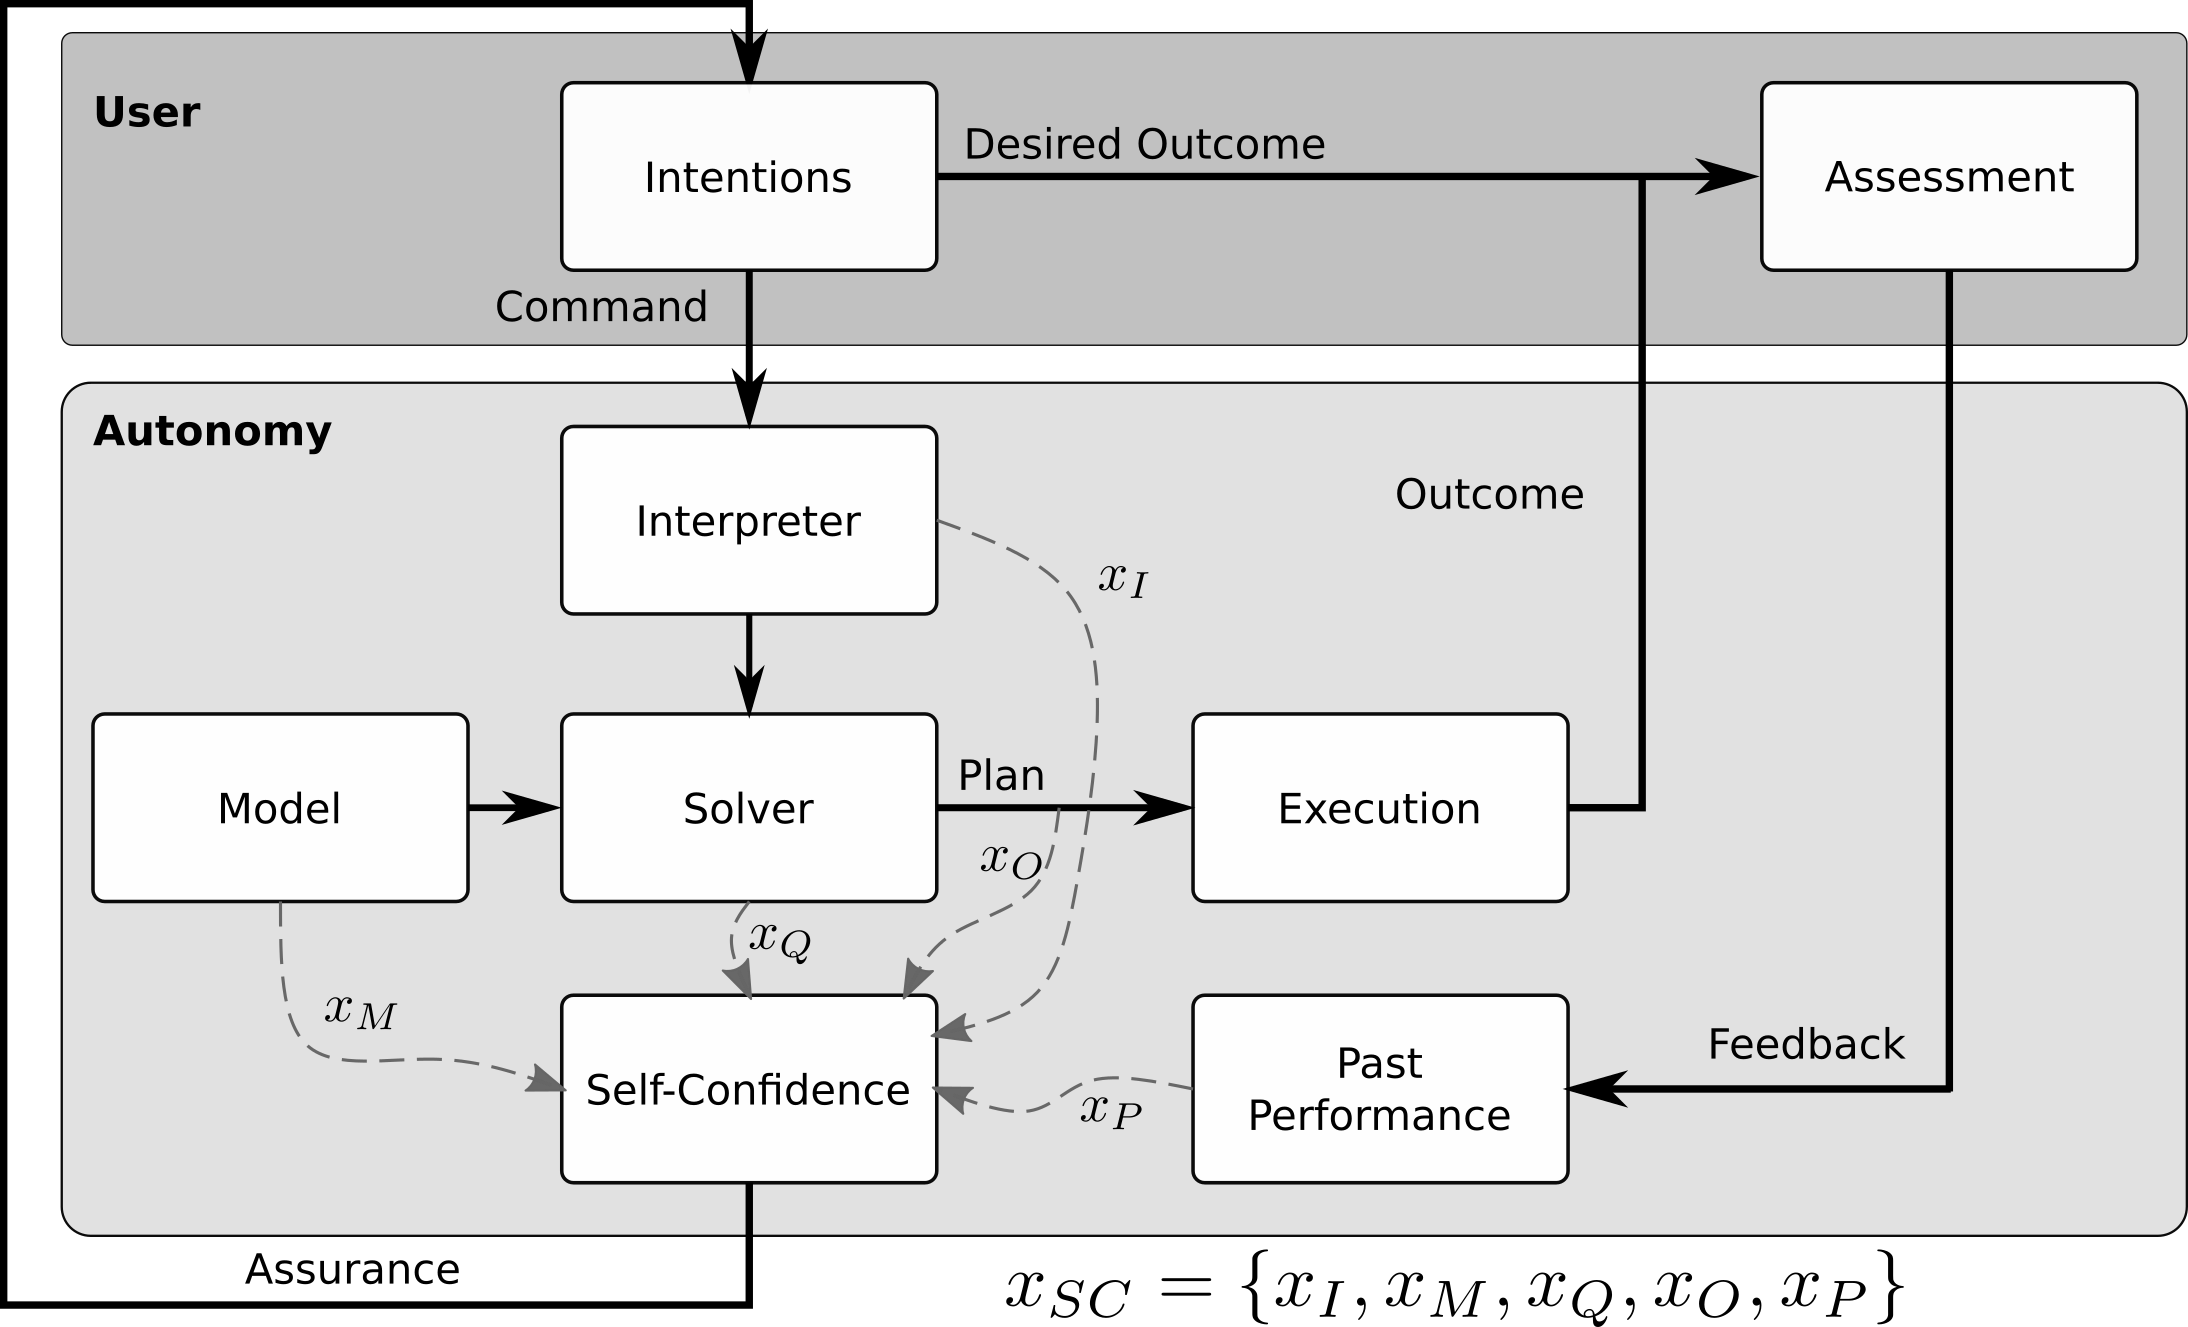
\includegraphics[width=0.6\linewidth]{Figures/FaMSeC.png}
        \caption{Factorized Machine Self-Confidence (\famsec) information flow}
        \label{fig:famsec}
    \end{figure}
    
    Figure \ref{fig:famsec} illustrates \famsec's notional overall self-confidence scoring mechanism. This uses a set of \emph{self-confidence factors} (dashed lines) that are derived from core algorithmic decision-making components (white boxes in the `Autonomy' block). The total self-confidence score can be mapped onto an arbitrary scale, e.g. -1 to +1 for the sake of discussion, where -1 gives a shorthand indication of `complete lack of confidence' (i.e. some aspect of task, environment, or context falls completely outside the system's competency boundaries), and +1 indicates `complete confidence' (i.e. all aspects of task, environment, and mission context are well within system's competency boundaries). As will be shown later, the scales for each factor need not all be the same and can carry slightly different qualitative interpretations, as long as a clear sense of `confidence direction' (i.e. degree of self-trust) can be established for each.
    
    Ref. \cite{Aitken2016-cv} considers five general factors that contribute to a `total self-confidence score', which notionally maps the combined set of factors into an overall confidence report:
    1) \xI---\textit{\textbf{interpretation of user intent and task}}: to what extent were the user's intentions properly understood and translated by the autonomous system into context-appropriate mission specifications and tasks?; 
    2) \xM---\textit{\textbf{model and data validity}}: are the agent's learned and/or assumed models, and training data used for decision-making `good enough' proxies for the real world?; 
    3) \xQ---\textit{\textbf{solver quality}}: are the approximations and learning-based adaptations used by the system for solving decision-making problems appropriate for the given mission and model?; 
    4) \xO---\textit{\textbf{expected outcome assessment}}: do the sets of possible events, rewards, costs, utilities, etc. for a particular decision lead to a desirable landscape of possible outcomes?; and 
    5) \xP---\textit{\textbf{past history and experiences}}: what can be gleaned from the system's own experience and other available information for past problem instances? %%\brett{refer to \cite{Israelsen2018-qz} for more detail if we feel we need it}

    Since the overall self-confidence mapping is heavily dependent on application, context, and desired levels/types of user-autonomy interaction, this work assumes for simplicity that the overall mapping consists of a direct report of all or some fixed subset of the component factors, e.g. \xSC. 
    Furthermore, the five factors considered here are neither exclusive nor exhaustive. For example, the factors developed by \cite{Aitken2016-cv} are primarily aimed at self-assessment \emph{prior} to the execution of a particular task, whereas it is conceivable that other self-confidence factors could be included to account for in situ and post hoc self-assessments. Attention is restricted here to the a priori self-assessment case. 

%\subsubsection{Revisiting Donut Delivery}
We will use the Donut Delivery problem to examine two core questions: (i) how should the factors be expected to behave under different conditions (independently of how they are actually calculated)?, and (ii) how should any one these factors actually be calculated?

For (i), we can first consider what kinds of trends, `boundary conditions', and which interactions are expected for the various factors if we are given some class of solver for the underlying ADT motion planning problem. For instance, if the problem were modeled and encoded as a discrete-time/discrete-space MDP, then sampling-based Monte Carlo solvers could be used to find an approximately optimal policy $\pi$ \cite{Browne2012-lj}, which would map joint ADT-MG state information onto specific actions to maximize the ADT's expected cumulative reward. Figure \ref{fig:trendsBCs} shows some expected behaviors for the \famsec{} factors for such a solver, as a function of task, environment, system, and context, assuming again an arbitrary finite range of -1 (total lack of confidence) to +1 (complete confidence). For instance, \xQ{} would be expected to increase/decrease as the number of samples used by the Monte Carlo solver to approximate $\pi$ increased/decreased. Similar trends can also be derived for other solver types.  %\nisar{mention about traceability/drill down basis here?}
\begin{figure}[tbp]
    \centering
    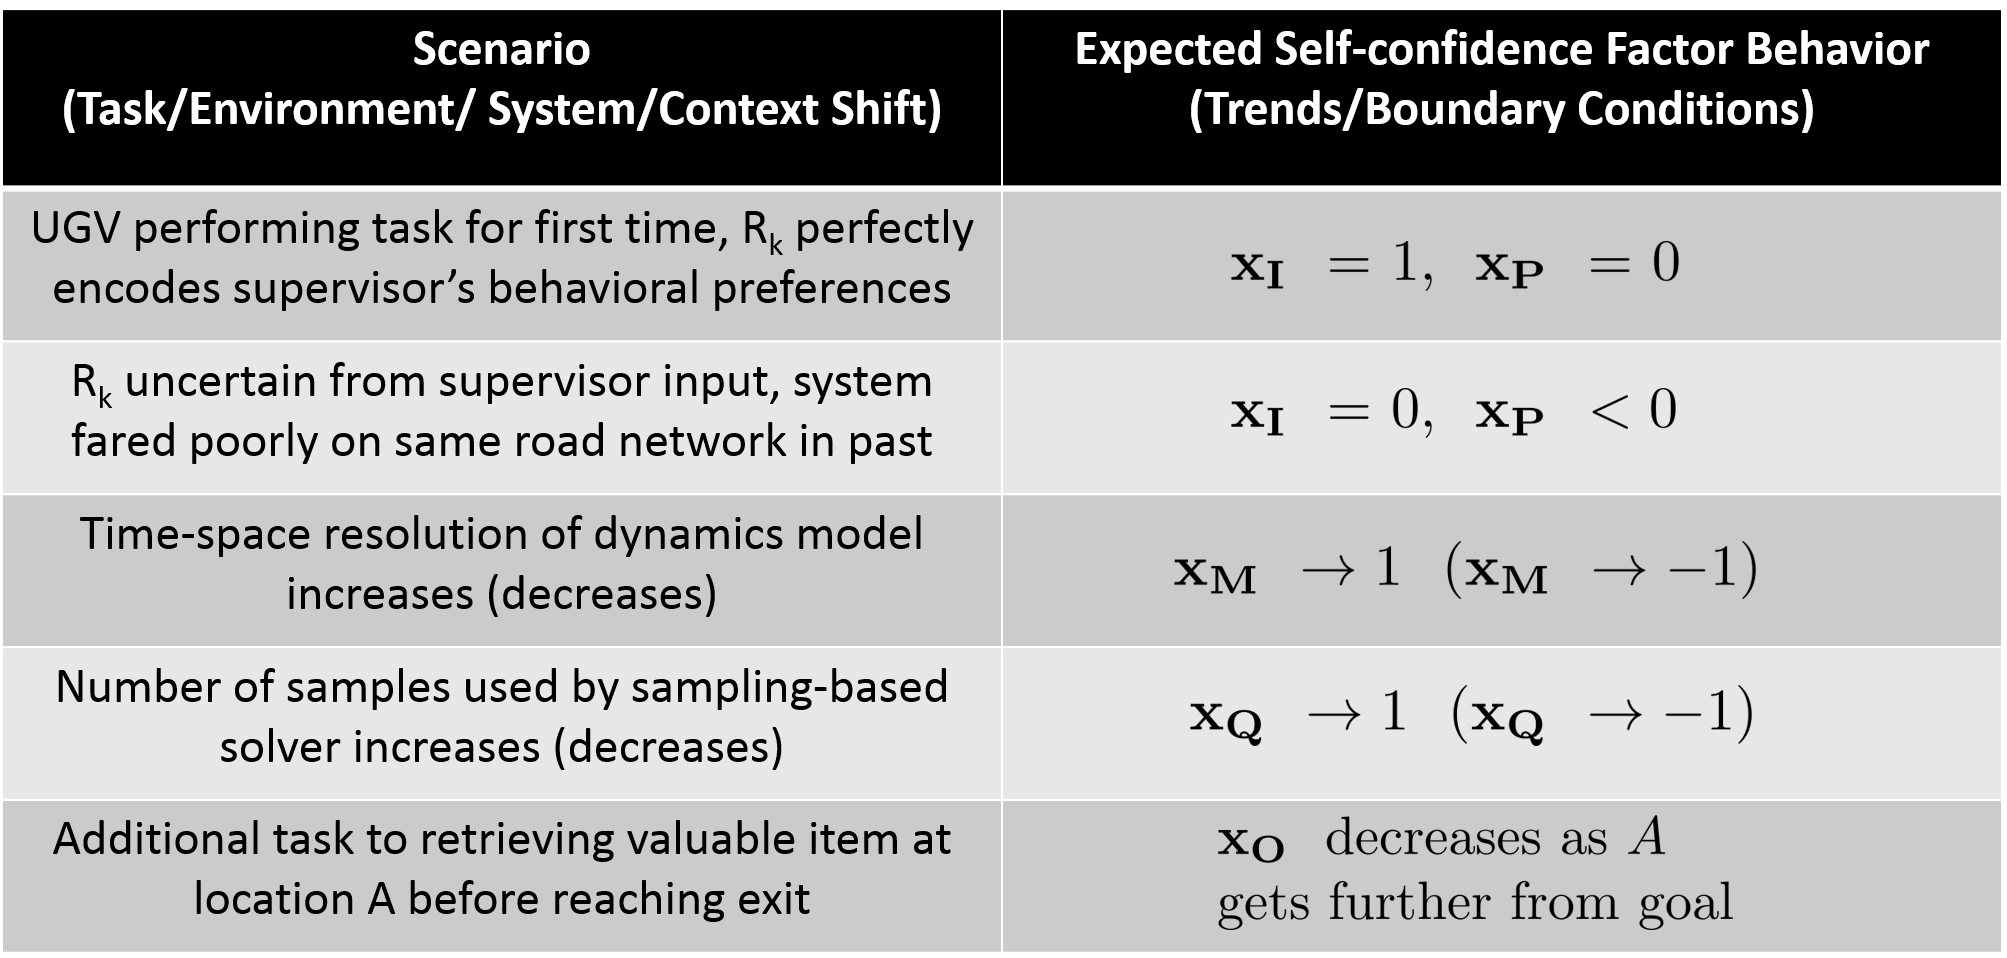
\includegraphics[width=0.65\linewidth]{Figures/scTrendsBoundaryExample_2generic.png}
    \caption{Notional \famsec{} factor behaviors for Donut Delivery problem.}
    \label{fig:trendsBCs}
\end{figure}

With this in mind, an important issue to consider for addressing (ii) is that the factors can depend on each other in complex ways. A logical simplifying assumption for initial algorithm development is to consider cases where we can ignore the interactions between factors. This is equivalent to examining each factor along `boundary conditions' where other factors do not change and thus have little/no contribution to the overall self-confidence score. 

However, ref. \cite{Aitken2016-cv} does not specify how to compute other factors, nor how to cope with interdependencies between factors that will arise when assumptions such as those above are relaxed. Furthermore, studies with human users have not yet been done to validate and evaluate the impact of self-confidence reporting on task delegation. The remainder of the paper addresses both gaps. 
